\chapter{Enjeux}

Pour aller vers l'optimisation de l'énergie, il nous faut prendre en compte sa création,
son transport, son stockage et sa consommation.
Le concept de Smart Grid permet d'apporter des éléments pour répondre à chacune de ces problématiques.

\section{Descriptif de la smart grid}
La smart grid est l'union de deux expertises, l'informatique et l'énergie.
Ce type de réseau permet l'échange d'informations sur l'état de la structure.
Ces connaissances sont importantes pour pouvoir optimiser la distribution, faire du stockage
et donc minimiser l'impact écologique de l'Homme.

L'un des intérêts de ce partage d'information est de pouvoir décentraliser la production d'énergie.
Tout point du réseau peut donc produire ou consommer son énergie.
Cette complexité supplémentaire nécessite de nombreux ajustements et changements de paradigme en terme de topologie.
L'un de ces changements est le coût de l'énergie. Celle-ci varie déjà aujourd’hui, mais cette variation
devrait être d'autant plus importante que les énergies renouvelables prendront une place forte dans
le mix énergétique citadin. Une solution serait que chaque ville possède une bourse de l'énergie
locale qui atténuerait les variations, et profiterait aux personnes consommant en heures creuses.

\begin{figure}[h]
    \centering
    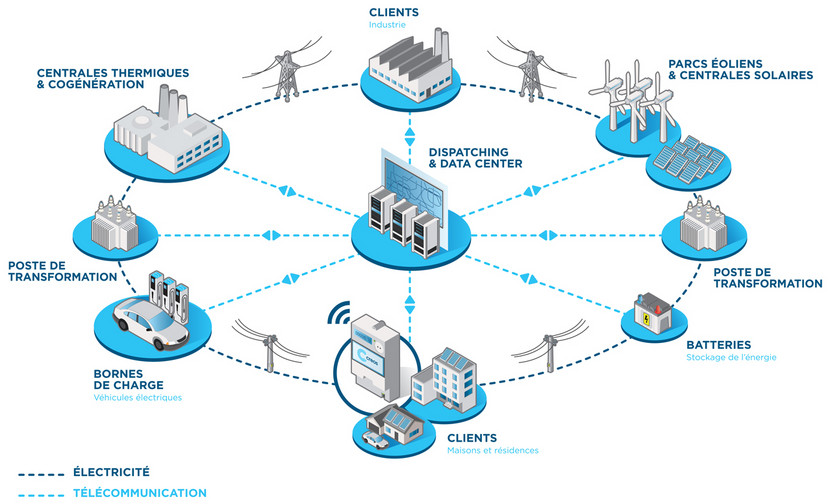
\includegraphics[scale=0.40]{media/smart_city_lux.jpg}
    \caption{
        Architecture d'une smartgrid\newline
        \tiny{Source: \url{https://www.creos-net.lu/creos-luxembourg/innovation/smart-grid/reseau-du-futur.html}}
    }
\end{figure}

% Micro grid

La microgrid est un autre type de réseau qui, contrairement à la smart grid, ne s'occupe pas de la communication.
Cette solution est envisagée plus sérieusement par de nombreuses communes pour des raisons de coût. En effet, ses
avantages restent nombreux tels que la gestion de différentes sources d'énergies opérées de manière parallèle,
ainsi qu'une fiabilisation du réseau déjà présent.

% https://www.researchgate.net/post/What_is_the_difference_between_a_microgrid_and_a_smartgrid
% A microgrid is an electrical system that includes multiple loads and distributed energy resources that can be operated in parallel with the
% broader utility grid or a Small, independent power system. It Increased reliability with distributed generation, Increase efficiency
% with reduced transmission length, and Easier integration of alternative energy sources.while
% A smart grid is a modernized electrical grid that uses information and communications technology to gather and act on information,
% such as information about the behaviors of suppliers and consumers, in an automated fashion to improve the efficiency, reliability,
% economics, and sustainability of the production and distribution of electricity. Transmission and operations: wide‐area monitoring,
% control and protection.


% Analyse des villes

\section{Villes connectées}
% Cette partie parlera de la partie technique de la mise en place de la smart grid
%   Ainsi que des différents problèmes que les villes actuelles ont.

Les villes intelligentes dites connectées essaient de répondre à quatre enjeux majeurs.
\begin{itemize}
    \item La connectivité des citoyens et de la ville. Il faut collecter et transporter un maximum d'informations dans les
deux sens pour optimiser les décisions et le bonheur de ses habitants.
    \item Des transports intelligents pour désengorger les rues et fluidifier le trafic.
    \item Une réduction des émissions de polluants dans l'environnement pour répondre aux enjeux du
réchauffement climatique.
    \item Un accompagnement du tourisme pour avoir un rayonnement international et attirer des entreprises.
\end{itemize}

\subsection{Connectivité}
% Cette partie parlera de la partie humaine de la connexion a la smart grid.
% ex. La 5G (6G) et les réseaux sociaux
%     Communication et report de problèmes
Il est possible de connecter toute la population et les services publics dans un
seul grand réseau lié à la smart city.
Sur la base d'un puissant réseau de fibres optiques et de la technologie Wi-Fi, Mesh et WiMAX,
avec une extension supplémentaire, un réseau sans fil à large bande peut être construit.

Dans le même temps, une station de base large sans fil couvrira toute la ville.
Et grâce à sa largeur de bande, elle peut assurer de nombreuses fonctions de gestion urbaine
et de systèmes de services pour le public, les entreprises, les visiteurs étrangers,
les touristes et les agences gouvernementales.

Ces fonctions comprennent la vidéosurveillance mobile sans fil, la vidéoconférence mobile,
la répartition mobile des interventions d'urgence et les télécommunications d'urgence.

\subsection{Transports}

En fonction de ses besoins et de la situation de la circulation,
chaque ville peut tirer profit du réseau de capteurs,
de l'Internet des objets ainsi que d'autres moyens techniques pour modifier le transport
traditionnel et mettre en place le système de gestion intelligente du trafic,
y compris les feux de signalisation adaptatifs (contrôle automatique de la circulation
feux en fonction du temps d'écoulement) système de contrôle, et ainsi de suite.

À ce stade, le trafic intelligent peut réaliser l'intégration des systèmes
de gestion urbaine la planification, la construction, la gestion et l'exploitation, et fournir
un soutien complet pour d'autres sous-systèmes de système urbain.

\subsection{Écologique}

Grâce à la technologie, nous pouvons réaliser non seulement la mise en réseau,
l'interopérabilité et le contrôle de divers appareils et systèmes, mais aussi la collecte,
la transmission, le stockage, l'affichage et le contrôle des données audio, vidéo et l'information d'alarme.
Dans le même temps, il peut également réaliser le lien avec le système d'alarme, et fournir
une interface de données pour d'autres systèmes.

Toutes ces données aideront les organismes compétents de la municipalité pour agir dans les meilleures
conditions. Les systèmes d'alarmes peuvent par exemple alerter en cas de fuite d'hydrocarbure dans
les systèmes d'approvisionnement.

\subsection{Tourisme}

Le tourisme intelligent est un moyen d'obtenir des informations sur les voyageurs.
Il devrait être basé sur les informations touristiques existantes et des infrastructures,
en tirant parti correctement de l'information numérique et l'Internet des objets pour parvenir
à la mise en place d'un ensemble de solutions, qui peuvent prendre en compte et remplir
la gestion et les tâches liées au tourisme.
Elles devraient prendre en compte
les services en ligne de tourisme,
la gestion de la relation client,
la gestion des développements du marché du tourisme intérieur et extérieur,
un système de gestion intelligent du moniteur,
de la collecte des informations touristiques
et les prévisions de développement du tourisme.

Ces données peuvent être mises à dispositions du marché du tourisme, et ainsi optimiser l'attractivité de la ville.
Cela implique des communications entre les services gouvernementaux, les services touristiques et les entreprises
pour promouvoir ce tourisme intélligent.

\subsection{Difficultés}

L'information spatiale de la ville intelligente provient d'une grande variété de capteurs,
de contrôleurs et de terminaux informatiques, et est entretenu par des ordinateurs et des nœuds
de stockage différents de l'équipement.
Comment gérer et coordonner l'équipement avec des structures variées et une large distribution sur
le territoire est le grand défi de la construction d'une plate-forme de services.

D'autre part, les informations sur la ville intelligente contiennent non
seulement une grande quantité de des données structurées, telles que la température, le voltage,
mais aussi beaucoup de données non structurées, sous forme d'images, de fichiers audio ou vidéo.

Il faut pouvoir stocker et gérer efficacement les énormes quantités de données sans affecter
les performances des services d'information.
Enfin, la ville est liée à l'analyse intelligente de l'information urbaine, l'aide à la décision,
les affaires publiques et de nombreuses autres applications.
Un grand nombre de tâches en temps réel doivent également répondre aux demandes des utilisateurs rapidement,
ce qui entraîne des exigences plus élevées en matière des services d'information.

Pour le caractère de services d'information et les problèmes non résolus,
nous devons étudier le système de service d'information urbain intelligent à tous les niveaux,
proposant des méthodes efficaces et efficientes, ce qui représente une large intégration des
dispositifs Internet, de la Big Data et d'un grand nombre d'utilisateurs.

\section{Les mutations de la ville}

Les urbanistes sont confrontés à la décision de la politique d'urbanisme à mener afin de réaliser le meilleur avenir possible.
De nombreuses villes des pays développés utilisent des modèles complets qui simulent divers aspects du système urbain,
capables de prédire les implications d'un ensemble donné d'apports politiques, afin d'aider le processus de planification.
Toutefois, dans les pays en développement, il est possible d'obtenir des données démographiques et socio-économiques
avec une extrapolation des données disponibles.
Cela limite le développement de modèles urbains aussi complets pour soutenir les décisions de planification.
En l'absence de modèles, le processus d'élaboration des plans tend généralement vers une approche plus intuitive.

Mettre en œuvre des politiques et des réglementations compactes en matière de croissance urbaine
permet une meilleure gestion des ressources de la ville.

Le développement urbain devrait chercher à obtenir une empreinte compacte en préservant les
espaces, la réutilisation et le remplissage des zones existantes, et l'expansion dense de la nouvelle croissance.
Une variété des outils réglementaires et incitatifs favorisant une croissance urbaine compacte sont disponibles
et doivent inclure :

\begin{itemize}
    \item Péage routier
    \item Gestion des espaces verts
    \item Réaménagement et conversion des friches industrielles et les sites en détresse des quartiers urbains
    \item Accélération des permis de projets
    \item Lignes directrices en matière d'urbanisme et de conception des rues qui illustrent la manière d'intégrer l'énergie
    les principes d'efficacité et d'habitabilité
    \item Gestion de la demande de transport, par exemple en réglementant le stationnement et en imposant l'usage de la route
\end{itemize}

Certains de ces outils de mise en œuvre nécessitent souvent l'adoption d'une législation voté
par les gouvernements avant leur introduction par les autorités locales.

L'intégration des infrastructures urbaines à l'environnement bâti a été de plus en plus
reconnue comme un moyen de renforcer la compétitivité économique des villes, d'améliorer
l'environnement et l'efficacité énergétique, et l'accroissement de l'équité sociale.

Les pôles de transport public bénéficient d'analyses de densité urbaine,
des services et des équipements. Il est fondamental de faire correspondre la densité urbaine et
les infrastructures si l'on veut que les villes ne soient pas submergées.
Les infrastructures doivent être à la hauteur de la densité de population et ne pas entraîner des encombrements.

Guidée par une vision qui met l'accent sur les principes de développement axés sur le transport,
Curitiba au Brésil a construit de nouveaux aménagements stratégiques le long de ses couloirs de transport
en commun rapide par autobus, et aujourd'hui, la ville a des niveaux d'émission de gaz à effet de serre plus
faibles, moins d'embouteillages et des espaces urbains plus agréables à vivre par rapport à d'autres
villes brésiliennes similaires.

Les modèles de croissance urbaine ont été largement façonnés par les forces du marché. Les deux villes
ont manqué une occasion d'aligner le développement urbain sur la capacité des transports en commun.

Les villes de demain se développeront autour des sources d'énergies qui sont à sa disposition.
La topologie idéale est

\begin{itemize}
    \item Une source d'énergie forte au centre telle qu'une centrale nucléaire
    \item Des industries lourdes autours de cette source d'énergie
    \item Des bureaux et des zones marchandes de grande densité autours des industries
    \item Des zones de vies en périphérie de la ville.
\end{itemize}

Chacune de ces zones doivent être équipées de moyens de transport efficaces pour
éviter toute congestion.

La topologie concentrique de cette ville permet une bonne répartition de la population.

\begin{SCfigure}[][h]
    \centering
    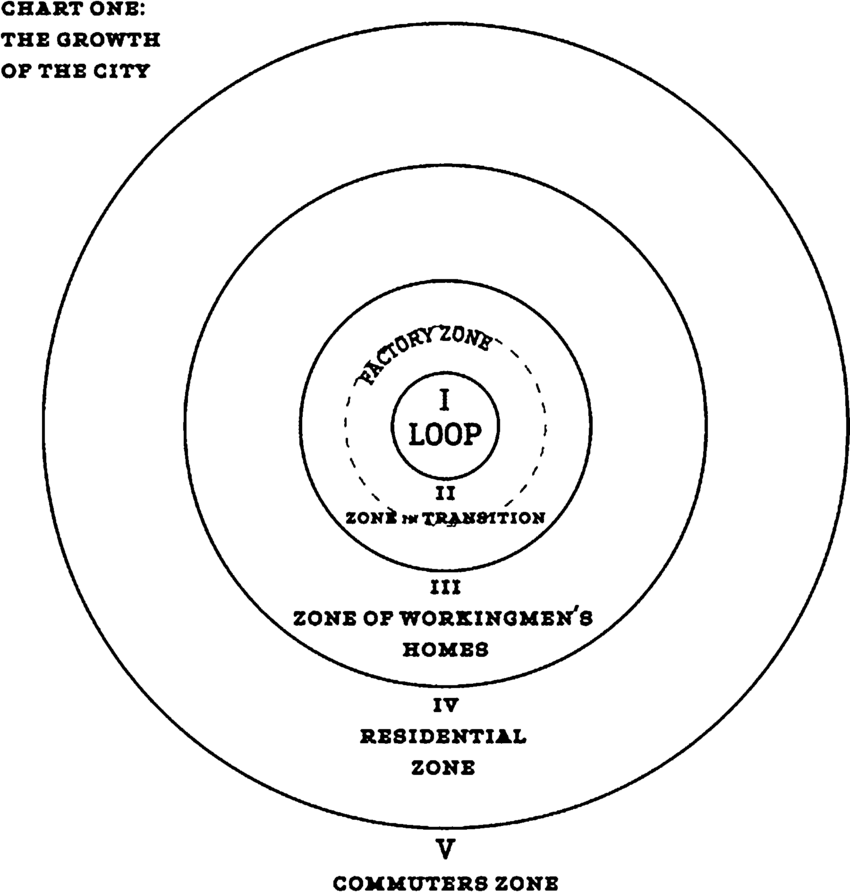
\includegraphics[scale=0.30]{media/Concentric-zone-theory-Source-Burgess-1925.png}
    \caption{
    Zone théorique Concentrique\newline
        \tiny{Source:\newline
          \url{https://www.researchgate.net/profile/Bhargav_Adhvaryu/publication/248512662/figure/fig4/AS:703689396346885@1544784034514/Concentric-zone-theory-Source-Burgess-1925.png}
        }
    }
    \label{fig:concentric-zone-theory}
\end{SCfigure}

Paris est un contre exemple de ville concentrique. En effet, due à des politiques d'exclusion des classes populaires,
l'Est et le Nord de Paris sont plus pauvres que l'Ouest et le Sud.
Dû à cette différence, le centre d'attache des entreprises se retrouve déplacé vers ces villes riches, de prestige,
et donc éloigné de la population.
L'hyper-centre de Paris est touristique et attire une masse de personnes ce qui rend difficile la coordination des
transports qui se doivent en majorité de passer par l'hyper-centre, ce qui donne un nombre important d'engorgements.

Les travaux du grand Paris essaient de gommer les erreurs de topologie en donnant à l'Est un plus grand nombre de moyens de
transport, ainsi que des aides aux entreprises pour s'y installer.

\section{Étude de cas - IssyGrid}

Le projet IssyGrid est un bon exemple de SmartGrid implantée en France.
Nous avons pris contact avec M. Alexandre CAPELLE, Directeur des Solutions Logicielles chez Embix pour
lui poser quelques questions sur le projet.
Ses réponses viennent compléter nos recherches sur le projet, tandis que son interview complète peut être
trouvée en annexe.
M. Eric LEGALE, directeur d’IssyMedia et chargé de la communication de la ville,
nous a également fourni quelques éléments de réponse sur les aspects sociales du projet.

\subsection{Présentation du projet}
Initié par Bouygues Immobilier, le projet a vue le jour en 2012 dans la ville d'Issy-les-Moulineaux,
commune française dans le département des Hauts-de-Seine.
Le projet fut bien accueilli et encouragé par le maire de la ville, André SANTINI.
En revanche, aucune aide financière ne fut apporté par la commune.

``Le projet a été financé exclusivement par le consortium, sans apport de la ville''
--  Éric LEGALE, directeur d’IssyMedia, chargé de la communication et
de l’innovation de la ville.

Le projet n'a pas impliqué qu'un seul acteur, mais un consortium de dix compagnies :
Bouygues Energies \& Services, Bouygues Immobilier, General Electric, EDF, ENEDIS, Microsoft,
Objenious, Schneider Electric, Sopra Steria et Total.

Ce sont eux qui ont financé le projet.
Pour joindre le consortium, un apport d'une valeur de 250 000€ était nécessaire.
Ce budget a permis ensuite de financer les recherches et les coûts matériels d'autres entreprises partenaires telles que Embix.
IssyGrid fut un terrain d'expérimentation.

L'expérience a duré 8 ans, et a un impact sur la vie de 5.000 habitants, 10.000 employés
et 160.000 m2 de bureaux sur deux quartiers de la ville, Bords-de-Seine (quartier des affaires),
puis Fort en 2015.

\begin{figure}[h]
    \centering
    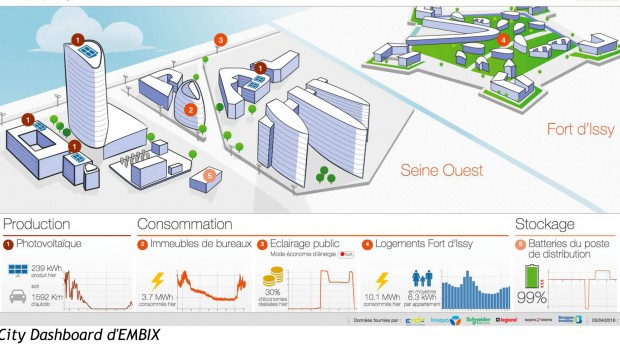
\includegraphics[scale=0.70]{media/issygrid.jpg}
    \caption{Le projet IssyGrid\newline
        \tiny{Source:
          \url{https://www.constructioncayola.com/reseaux/article/2016/05/20/105695/issygrid-quartier-reseau-malin}
        }
    }
\end{figure}


Le projet a fait face à plusieurs types de défis.

\subsection{La collecte de données}
Tout d'abord un défi quant à la collecte des données des différentes infrastructures.
Les informations de consommation d'énergie et de déplacements sont essentielles pour que la ville
puisse s'adapter à sa population.

L'entreprise Embix a été créée en 2011 par Bouygues Immobilier, Bouygues Energie et Service, et General Électric,
à l'occasion du projet en réflexion. Sa mission fut de répondre
à cette problématique en instrumentant la ville de capteurs
capables de récolter des informations telles que la température, la consommation de chauffage, d'électricité,
la qualité de l'air\dots

Tout d'abord sur les bâtiments du tertiaire.
Les capteurs ne sont pas directement connéctés à Internet, mais sont capables de communiquer entre eux
via un réseau filaire et des protocoles tels que Modbus et BACnet.
Ces données sont traités par un outils GPB - Google Protocol Buffers - qui permet de traduire des données
issus de divers formats de communication. Elles sont rendue publiques sur Internet par la GPB.

Ensuite sur les bâtiments résidentiels. Pour chaque logement, les capteurs sont reliés en filaire à un compteur
qui lui est connecté à Internet.
Le projet est parvenu à un accord sans précédent avec la CNIL :
la collecte des données est autorisée par lot de dix habitations afin de conserver son anonymat et garantir
la confidentialité particulière d'un logement.
D'autant plus que la ville a choisi de faire de l'Open Data.
Chaque foyer doit toutefois donner son accord pour que ses données alimente le flux.

Les compteurs Linky, dont sont équipés les logements récents, permettent de communiquer les informations
de consommation d'éléctricité auprès de ENEDIS.
Les données journalières récoltées par leur serveurs sont donc stockées sur leurs serveurs.
La création de ces appareils répond à une directive européenne,
mais ils ont utilisé les Eco-quartiers comme terrains de test.
Il existe l'équivalent du compteur Linky pour la consommation de gaz : son cousin Gazpar.

Il existe un dernier type de réseau sur les bâtiments de la ville.
Il y a par exemple un objet connecté branché sur le compteur de la gare RER capable de
communiquer les données via le réseau longue portée LoRa qui couvre déjà le territoire français.
Il n'y a donc pas besoin câbles, ces objets connectés réutilisent un réseau d'ondes radio déjà mis en place par Bouygues Télécom.


\subsection{Un défi technique}

La collecte de données fut un défi technique à part entière.
Tous les capteurs de la villes communiquent en effet via des protocoles de communication différents.
Pour qu'Embix puisse créer un centre d'analyse et d'optimisation, ils ont dû apprendre
à communiquer avec une quinzaine de protocoles différents puisqu'il n'existait aucune standardisation.

Mais ce projet de R\&D a aussi permis de faire plein d'innovations.

Total a par exemple fait des progrès sur le raccordement des panneaux photovoltaïques.
L'énergie créée en trop lors des heures creuses est stockée dans des volants d'inertie et dans des
batteries. Un accord a été passé avec Renault pour récupérer leurs anciennes batteries de voitures
électriques, démontrées comme suffisantes pour les quartiers Isséens.

Dans une des tours du quartier des affaires, il a fallut répondre à un problématique de climatisation
dont la consommation était très importante en été.
Un nouveau système de "pile à froid" a été imaginé.
La nuit, durant les heures creuses, l'éléctricité est sollicitée pour créer un grand bloc de glace.
En journée, plutôt que de faire tourner la climatisation à plein régime, on fait
fondre ce bloc de glace pour recréer de l'électricité.

D'autres éléments déjà largement utilisés dans les villes ont aussi été mis en place dans IssyGrid.
Bouygues Energies \& Services a par exemple travaillé sur l'éclairage urbain pour que les réverbères
consomment moins d'énergie et lutter contre la pollution lumineuse. Ils sont capables d'adapter
leur éclairage en fonction de l'heure et des présences à proximité.

\subsection{La communication}
Un autre défi majeur fut la communication.
Tout au long du projet, la ville a fait un éffort de vulgarisation du projet afin de rassurer
la population par divers moyens de communication et de modules pédagogiques. La population a accès
a une interface pour suivre la consommation et la production d'énergie en temps réel grâce à des
graphes simples et intuitifs afin de la sensibiliser et la rendre actrice du projet.

Nous avons intérrogé M. Eric LEGALE, qui nous a confirmé que le projet n'a rencontré aucune opposition.

Un autre aspect de ce défi fut la communication entre tous les acteurs du projet.
Ces acteurs issus du public et du privé n'avaient en effet pas tous l'habitude de travailler
dans un projet réunissant autant de collaborateurs et partenaires.


\subsection{SWAYS et Galéo - Des exemples de bâtiment du tertiaire}
SWAYS - Smart Ways to work - est un immeuble de travail de l'éco-quartier des affaires de IssyGrid.
Tout est fait pour améliorer le confort des utilisateurs.
Il privilégie un éclairage naturel dans les bureaux et la purification de l'air par la biophilie,
le tout grâce à un toit végétale. Des commerces de proximité et autres structures de loisir
sont installés à l'intérieur même du bâtiment. D'un point de vue technique, le bâtiment serait
capable d'anticiper les pannes grâce à de la maintenance prédictive, assure une couverture réseau
4G dans tout le complexe, et propose même aux utilisateurs des applications liées à l'activité du
bâtiment, ainsi qu'une cyber sécurité renforcée.

M. Alexandre CAPELLE nous a parlé du bâtiment Galéo, siège de Bouygues Immobilier.
Le fait d'instrumentaliser le bâtiment leur a permis d'améliorer progressivement le confort.
Ils ont par exemple remarqué que la qualité de l'air se dégradait dans les salles de réunion après un certain temps.
Et sur le plan thermique, de détecter les fuites de chaleur.
Leur façon de travailler n'a donc pas changé drastiquement, mais leur confort s'en est trouvé amélioré.
Le confort n'est donc pas incompatible avec l'économie d'énergie.

\subsection{SoMobility}
IssyGrid est un projet de SmartGrid. Son but est d'optimiser l'énergie dans la ville.
Mais ce qu'il faut savoir, c'est que ce n'est pas le seul projet dans la ville de Issy-les-Moulineaux.
Il y a effectivement un projet de Smart City avec le projet SoMobility, géré par un consortium composé de
la ville, du Groupe Caisse des Dépôts, Cisco, Bouygues Immobilier, Transdev et Colas, et réunissant au total plus de 40 acteurs.

Ils ont pour ambition de fluidifier la circulation dans la ville.
Ils ont pour cela quelques idées :
\begin{itemize}
    \item Rendre les feux tricolores plus intelligents et capables de prendre des initiatives ;
    \item Utiliser l'Open Data pour afficher sur des cartes le trafic en temps réel ;
    \item Indiquer les places disponibles aux conducteurs, toujours via des applications ;
    \item Déployer des mini-bus sans chauffeur dans la ville ;
\end{itemize}

Au delà des ressources techniques mises en place, les habitants sont aussi sensibilisés à travailler
dans des espaces de coworking avant d'aller au bureau afin de désengorger les routes et transports
en commun, et le covoiturage est aussi mis en avant.

\subsection{Bilan}
Le bilan de IssyGrid a été présenté en juin 2019.
Il ne présente malheureusement pas de chiffres pour ces six années de test, mais annonce en revanche
ses objectifs pour 2020 : ``Une efficacité énergétique accrue de 20 \%, une réduction de 20 \%
de l’empreinte carbone et une part de 20 \% des énergies renouvelables dans la production
énergétique européenne.''

Les chiffres d'IssyGrid n'ont pas été communiqués, mais un témoignage de Gironde HABITAT nous indique
que l'économie générée sur la consommation énergétique serait au mieux de 60€ par an à l'échelle d'un
foyer.

La ville d'Issy-les-Moulineaux souhaite agrandir la Smart Grid à un troisième quartier
``Issy Coeur de Ville''.
D'autres villes s'inspire d'IssyGrid. La ville de Nanterre par exemple a décidé de lancer un projet
d'éco-quartier également. Mais il rayonne aussi à l'international : des délégations
chinoises et japonaises viennent s'informer du projet.
C'est après tout un projet qui a duré 8 ans et dont on peut tirer beaucoup de leçons,
alors qu'un projet de ce genre dure généralement entre 3 et 4 ans.

Nous avons demandé à M. Alexandre CAPELLE quelles étaient ces leçons.
Entre ce qui différencierait une structure d'aujourd'hui a une structure montée 5 ans auparavant,
ce serait avant tout la complexité du projet.
Ils ont dépensé beaucoup d'effort dans la recherche de l'opposition avec des algorithmes avancés
et de l'intelligence artificielle, mais ils se sont rendus compte qu'une grande partie de
l'optimisation pouvait être faite assez simplement en instrumentant les bâtiments.
Sans faire de calculs compliqués de prédiction, la simple analyse de données est suffisamment
révélatrice pour corriger une bonne partie des pertes d'énergie.


\section{Des projets en échec}

Lors de la VivaTech Paris 2019, Emmanuel BAVIERE (Société Générale), Erwan KERYER (KPMG)
et Jérôme MONCEAUX (SPOON) ont pris la parole le vendredi 16 mai pour expliquer le phénomène autour des
Smart Grid. Un terme fort a été employé durant cette prise de parole :
``La Smart City ne marche pas''.

En se basant sur plusieurs exemples de projets en échec, divers arguments à ce propos ont été mis en
avant :
\begin{itemize}
    \item Des projets trop ambitieux ;
    \item Un manque de communication avec la population qui fait face à une puissance effrayante car mal comprise ;
    \item Les grands groupes ne savent pas comment gérer les tensions et désaccords avec les élus et la population ;
    \item Un manque de formation de la population qui ne sait pas utiliser les nouvelles technologies ;
    \item Une population qui refuse de partager ses données pourtant nécessaires au bon fonctionnement d’une Smart Grid ;
    \item Le gouffre séparant les populations aisées des populations pauvres s'élargie.
\end{itemize}
Bien qu'ils parlaient de Smart City et non de Smart Grid, ces éléments sont tout aussi importants dans les deux cas.

Le projet Smart City Quayside de Toronto réunit la plupart de ces éléments alors qu'il est encore en phase d'instruction.
Le projet n'est porté que par une seule entreprise, Sidewalk Labs, une filière de Google.
Celui-ci a été réfléchi pendant 18 mois avant de proposer un plan d'action de plus de 1 500 pages.
Les oppositions au projet sont multiples. On lui reproche avant tout son manque de démocratie.
Mme. Bianca WYLIE, figure de l'opposition, accuse les grands groupes derrière le projet de vouloir noyer l'information
avec la publication d'un document aussi volumineux auprès de la population.
De plus, le fait que de savoir Google derrière le projet ne rassure pas la population quant à la confidentialité des données.

En terme de Smart Grid, il existe assez peu de projets en échec.
